\subsection{Introduction}
The main application of the project is an Android app built on Unity. This allows the creation of a VR environment with ease. The only problem that arises from this choice is that it isn't possible to retrieve the data from the biosensor and send them to the smartphone directly as Unity doesn't allow a direct communication. As shown in figure \ref{fig:communication} the information from the biosensor are read first by a Computer and then sent to a Firebase server that stores the values. This values are then read by the Android application using a HTTP request.
\begin{figure}[h]
	\centering
	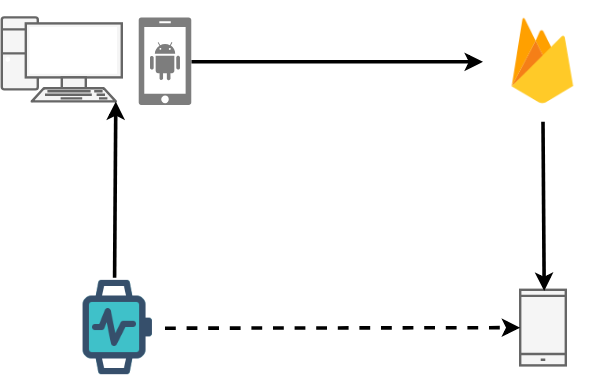
\includegraphics[scale=0.7]{ConnectionDiagram}
	\caption{Diagram that shows how the communication from the biosensor to the smartphone works.}\label{fig:communication}
\end{figure}

\subsection{Android Application}
Language used: C\#\\
Plugins:
\begin{itemize}
	\item ZXing
	\item Android Runtime Permissions
\end{itemize}

\subsection{Computer Client}
Language used: Java\\
Plugins:
\begin{itemize}
	\item ZXing
	\item JavaFX
\end{itemize}

\subsubsection{Description}
The computer client main task is to retrieve data from the Empatica E4 and send the values to the Firebase server. In order to do this, it communicates with E4 streaming server, an application that allows to forward realtime data of multiple Empatica E4 devices to multiple TCP socket connections.\\
The E4 Streaming server works through a message protocol where client request are in the following format:
\begin{center}
	COMMAND ARGUMENT\_LIST
\end{center}
Messages from server containing responses to commands are in the following format
\begin{center}
	COMMAND ARGUMENT\_LIST
\end{center}
Messages from server containing data from device are in the following format
\begin{center}
	STREAM\_TYPE TIMESTAMP DATA
\end{center}
The commands used from the client are:
\begin{itemize}
	\item device\_list\\
	requests the list of Empatica E4 devices to the E4 Streaming server
	\item device\_connect DEVICE\_ID\\
	sends a connection request to a specific device
	\item device\_subscribe STREAM STATUS\\
	start or stop receiving data from a given stream.
	\item device\_disconnect\\
	sends a device disconnection request
\end{itemize}
\pagebreak
\subsubsection{Algorithm design}
\begin{figure}[H]
	\centering
	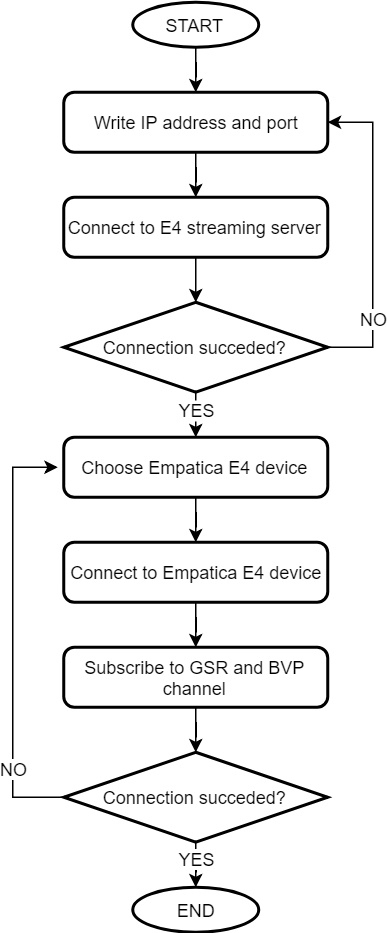
\includegraphics[scale=0.5]{BiosensorConnectDiagram}
	\caption{Flowchart that describes how the connection to the Empatica E4 device works}
\end{figure}

\begin{figure}[H]
	\centering
	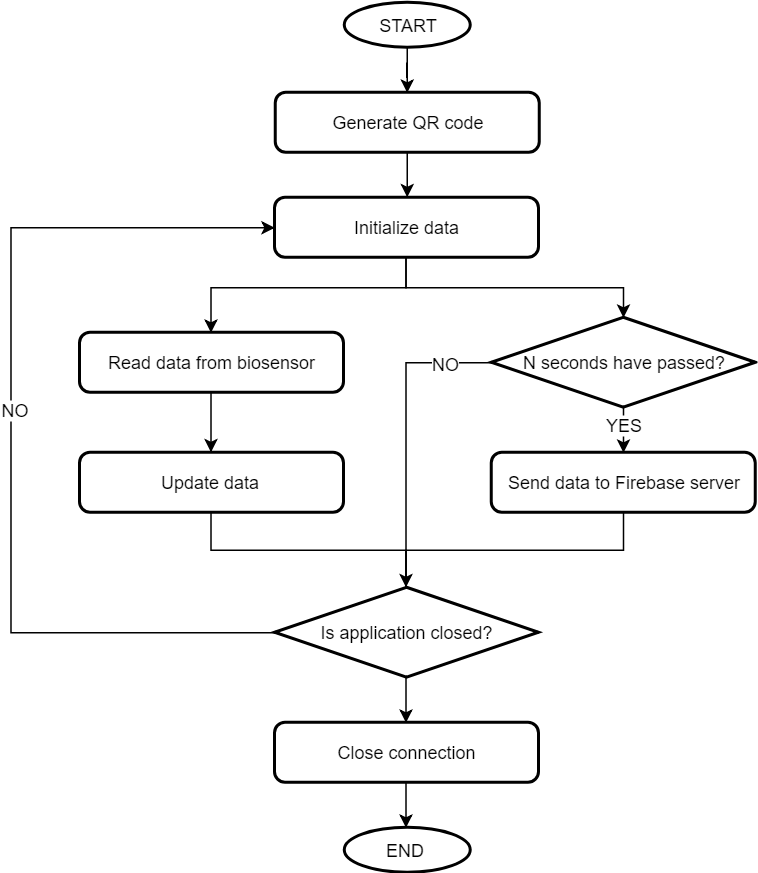
\includegraphics[scale=0.55]{BiosensorDataDiagram}
	\caption{Flowchart that describes how the client retrieve data from the Empatica E4}
\end{figure}

